\documentclass{ezb}
\usepackage[]{todonotes}
\usepackage{amsmath}
\usepackage{gensymb}
\usepackage{wrapfig}
\usepackage{longtable}
\usepackage[colorlinks,        	% Links ohne Umrandungen in zu wählender Farbe
   linkcolor=black,   			% Farbe interner Verweise
   filecolor=black,   			% Farbe externer Verweise
   citecolor=black    			% Farbe von Zitaten
]{hyperref}
\usepackage{booktabs}

\renewcommand{\thesubsection}{\alph{subsection}}
\begin{document}

% \maketitle{Nummer}{Abgabedatum}{Tutor-Name}{Gruppennummer}
%           {Teilnehmer 1}{Teilnehmer 2}{Teilnehmer 3}
\maketitle{22.05.15}{Udo Frese}{1}{Annika Ofenloch - 2992807 - ofenloch@uni-bremen.de}{Frank Ihle - 3010158 - fihle@uni-bremen.de}{Simon Schirrmacher - 4000884 - simons@informatik.uni-bremen.de}{Noshaba Cheema - ncheema@uni-bremen.de}

%-------Text-Start------------------------------------------
\section{Cutting-Edge Technology (10 Punkte)}

\begin{lstlisting}[language=C++, caption=]

\end{lstlisting}

\newpage
\section{Spargelzeit (4 Punkte)}
Unter Verwendung der Bildverarbeitung soll eine optische Qualitätskontrolle von Spargel durchgeführt werden. Zudem soll unter Berücksichtigung der Spargelqualitätsnorm UNECE-FFV-04 eine Sortierung in die jeweiligen Güteklassen erfolgen.

\subsubsection*{Zuführung des Spargels}
Nachdem der Spargel gewaschen und zugeschnitten wurde, wird er von Mitarbeitern auf ein Fließband abgelegt. Als Annahme wird getroffen, dass der Spargel immer gleich ausgerichtet ist und sich der Spargelkopf oberhalb des Fließbandes befindet. Als nächstes wird der Spargel zu sogenannten Sortierschalen transportiert, indem jeder Spargel separat vom Fließband in eine Sortierschale fällt (siehe Abbildung~\ref{fig:fliessband} und \ref{fig:sortierschale}). Von Mitarbeitern wird nachkontrolliert, ob sich auch wirklich nur ein Spargel in der Schale befindet oder ob ein Spargel daneben gefallen ist. Nicht befüllte Sortierschalen können vorkommen. Sobald sich der Spargel in den Sortierschalen befindet, wird dieser in ein geschlossen System transportiert, wo die Merkmalskontrolle unter Verwendung von Bildverarbeitung durchgeführt wird.
\begin{figure}[!h]
	\begin{center}
		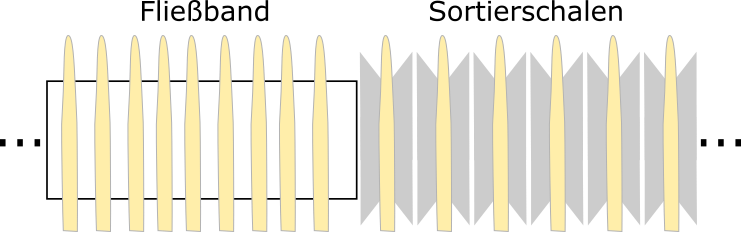
\includegraphics[scale=1.0]{fliessband_zu_sortierschalen.png}
	\end{center}
	\caption{Spargel fällt vom Fließband in den Sortierschalen}
	\label{fig:fliessband}
\end{figure}

\begin{figure}[!h]
	\begin{center}
		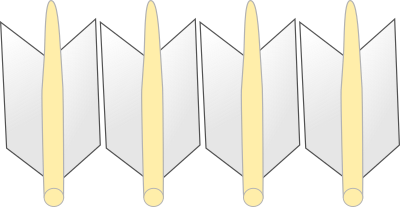
\includegraphics[scale=1.0]{sortierschalen.png}
	\end{center}
	\caption{Spargel in den Sortierschalen}
	\label{fig:sortierschale}
\end{figure}

\subsubsection*{Kamera und Umgebung}
Für die Merkmalskontrolle soll eine Bildaufnahme vom Spargel gemacht werden, wo keine Schattenwürfe oder andere externe Lichteffekte vorhanden sind, da solche Effekte als Schmutz oder Druckstellen interpretiert werden könnten. Die Lichtquelle selbst sollte nah bei der Kamera platziert werden, um einen Schattenwurf zu vermeiden (ggf. mehrere Lichtquellen oder ein Flächenlicht).\\
\begin{wrapfigure}{r}{0.31\textwidth}
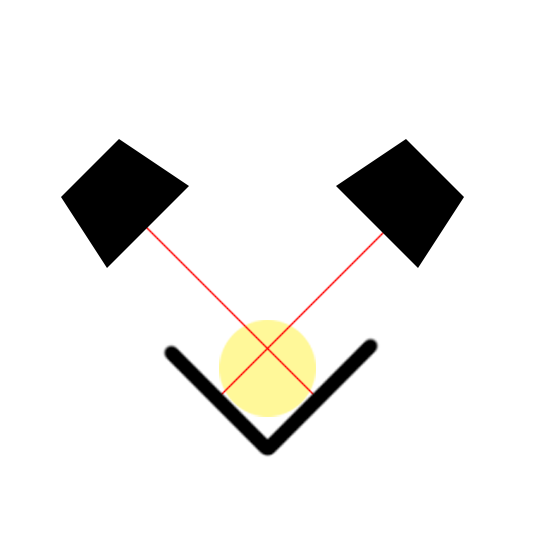
\includegraphics[width=0.25\textwidth]{kameras.png}
\caption{\label{fig:kameras}Positionierung der Kameras über den Sortierschalen.}
\end{wrapfigure}
Innerhalb des geschlossenen Systems, wo die Bildverarbeitung zum Einsatz kommt, werden zwei Kameras verwendet, die sich über den Spargelschalen und im Winkel von 90$\degree$ zueinander, in Blickrichtung der Schalenflächen ausgerichtet befinden (s. Abb. \ref{fig:kameras}). Die Kameras nehmen synchron einen definierten Bereich auf, der eine Sortierschale umfasst.
\clearpage
\subsubsection*{Fehler- und Merkmalskontrolle}
Mit Hilfe der Bildverarbeitung sollen die Merkmale Länge, Durchmesser, Farbe sowie Form des Spargels kontrolliert werden. Es werden zwei Aufnahmen gemacht.

Als erstes in der Ausgangsposition und wenn der Spargel um 90$\degree$ gedreht wurde (Der Spargel bleibt in den Sortierschalen und der herausragende Teil des Spargels wird auf einer Drehablage aufgelegt, sodass der Spargel gedreht werden kann).

Durch die zwei Aufnahmen kann der Spargel von zwei Perspektiven aus betrachtet werden, um Form und Durchmesser zu vergleichen als auch den Spargel gegebenenfalls auf weitere Druckstellen, Verfärbungen und Verschmutzen zu untersuchen.

Auf einer RGB-Bildaufnahme befinden sich acht Spargel, sodass vorerst eine Regionenbildung erfolgen muss. Betrachtet man die Aufnahme als Grauwertbild, unterscheiden sich die Grauwerte von den Sortierschalen (dunkle Grauwerte) zu denen des Spargels (helle Grauwerte). Demzufolge kann ein automatischer Schwellwert mit Hilfe des Otsu-Agorithmus festgelegt werden, sodass anschließend eine Regionenbildung unter Verwendung des Union-Region-Algorithmus durchgeführt werden kann.\\
\linebreak 
Als nächstes wird der Spargel separat in seiner jeweiligen Region betrachtet, um die Qualitätsanforderungen zu kontrollieren. Für die Merkmalskontrolle wird die RGB-Aufnahme verwendet. Anhand der Spargel-Länge und der runden Spargelspitze wird kontrolliert, ob dieser ganz ist. Die Rundung könnte unter Verwendung eines Kantenerkennungs-Algorithmus geprüft werden. Wenn keine Krümmung (Abgerundeter Kopf) vorhanden ist, wird der Spargel als unvollständig gekennzeichnet und demnach einen entsprechenden Ausgang (z.B. \glqq Fehlerhafter Spargel\grqq) zugeordnet. \todo[inline]{Wie wird der Spargelkopf erkannt?}
Die gesundheitliche und äußere Beschaffenheit des Spargels wird über eine Farbsegmentierung geprüft, indem braune als auch schwarze Verfärbungen betrachtet werden. Sobald der braune beziehungsweise schwarze Farbanteil einen prozentualen Anteil übersteigt, ist der Spargel krank, verschmutzt oder von Schädlingen befallen. Rostflecken und rosafarbige Verfärbungen lassen sich ebenfalls mit einer Farbsegmentierung erkennen.\\
\linebreak
Die Feuchtigkeit lässt sich mit Einschränkungen über eine Farbsegementierung überprüfen, da Wasserreflexionen zu weißen Flecken führen. Demnach kann der weiße Farbanteil näher betrachtet werden. Diese Variante funktioniert gut bei einem grünen Spargel. Bei einem weißen Spargel wird die Erkennung von Wasserflecken schwierig, da bereits ein hoher weißer Farbanteil vorhanden ist. Die Feuchtigkeit muss demnach mit einem zusätzlichen Ansatz geprüft werden, da die Bildverarbeitung hier an ihre Grenzen kommt. Das gleiche gilt für den Geruch, Geschmack und Prallheitsgrad, welche sich nicht mit der Bildverarbeitung kontrollieren lassen.\todo[inline]{spargel/hauptträgheitsachsen/regionen bild muss verschoben werden.}
\begin{wrapfigure}{r}{0.5\textwidth}
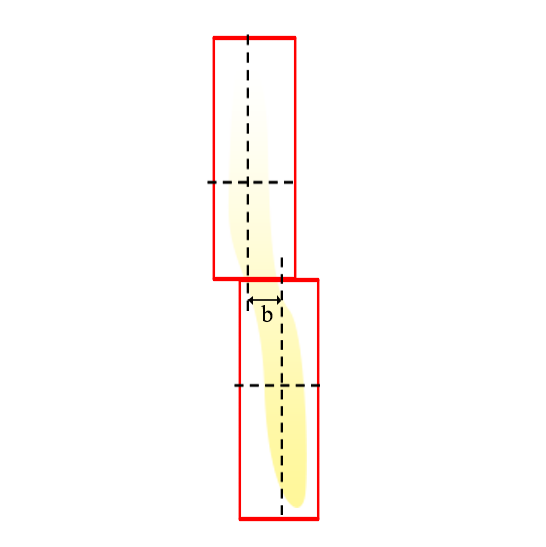
\includegraphics[width=0.5\textwidth]{schief.png}
\caption{\label{fig:schief}Der Spargel wird in zwei Regionen aufgeteilt, um so ein sicheres Ergebnis zu ermitteln.}
\end{wrapfigure}
Der Spargel wird in zwei gleichgroße Bereich aufgeteilt, von denen einzeln die Hauptträgheitsachsen ermittelt werden.(s. Abbildung \ref{fig:schief})
Anhand des horizontalen Abstands b der vertikalen Achsen kann erkannt werden, ob der Spargel zu krumm ist.
\clearpage
Ein weiteres Merkmal, das betrachtet werden soll, ist die Schnittfläche am unteren Ende des Spargels. Das abgeschnittene Spargelende muss glatt sein.\\
\begin{wrapfigure}{r}{0.5\textwidth}
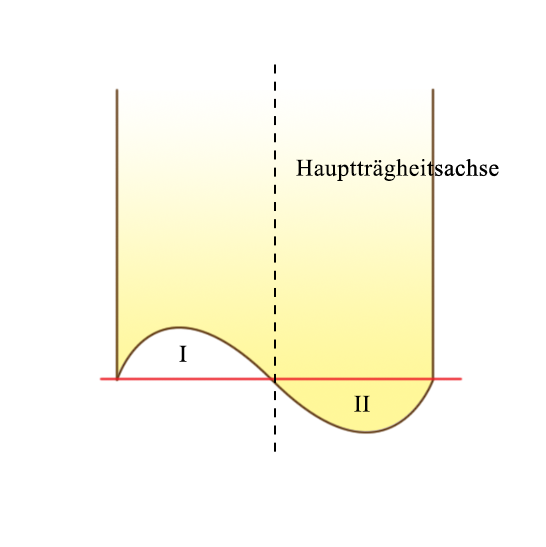
\includegraphics[width=0.4\textwidth]{schnitt.png}
\caption{\label{fig:schnitt}Die Schnittkante mit den genannten Flächen, die zur Qualitätseinteilung dienen.}
\end{wrapfigure}
Hierfür wird vom Schwerpunkt aus, entlang der Hauptträgheitsachse, die Schnittkante am Wurzelende des Spargels gesucht und der letzte Pixel des Spargels definiert.
Anhand von diesem gefundenen Pixel wird nun orthogonal zur Hauptträgheitsachse eine Gerade gezeichnet, mit der  die Qualität der Schnittkante überprüft werden soll.
Nun werden die Flächen ober- und unterhalb (I, II) der gezeichneten Orthogonalen mit Hilfe eines Integrals berechnet (s. Abb. \ref{fig:schnitt}).
Überschreitet diese Fläche einen bestimmten Schwellwert, ist die Qualitätsanforderung der Schnittkante des Spargels nicht erreicht.\\
\linebreak
Bei den zwei zuvor beschriebenen Verfahren ist es besonders wichtig, beide erzeugten Bilder auszuwerten, um auszuschließen, dass Qualitätsmängel aus einer Perspektive nicht zu erkennen sind.\\
\linebreak
Für die Größensortierung wird zusätzlich zur Länge noch der Durchmesser benötigt, der in der Spargelmitte, bezogen auf die Länge, ermittelt werden soll. Hierfür wird eine Gerade in Richtung der Hauptträgkeitsachsen (entlang der Breite des Spargels) bis zur Kante gezeichnet. Berechnet wird der Durchmesser für beide Bildaufnahmen (erforderlich bei einem ovalen Spargel). Für die Größensortierung (nach dem Durchmesser) wird der größere Durchmesser betrachtet.

Jede Sortierschale bekommt im Verlauf der Qualitätskontrolle einen entsprechenden Ausgang zugeordnet, der sich auf die einzelnen Qualitäts- und Größenklassen bezieht.

\subsubsection*{Sortierung des Spargels}
Der Spargel bleibt vom Übergabebereich des Fließbandes bis zu dem vom Bildverarbeitungssystem zugewiesenen Ausgang in der Sortierschale. Über die Merkmalskontrolle bekommt jede Sortierschale eindeutig einen Ausgang zugewiesen. Bei den Ausgängen handelt es sich um verschiedene Auffangbehälter, wo der Spargel je nach Qualitätsbestimmung
hin transportiert wird. Die Auffangbehälter stellen die einzelnen Qualitäts- sowie Größenklassen dar. 
Sobald die Sortierschale mit dem Spargel den zugehörigen Auffangbehälter erreicht
hat, kippt sich die Schale, sodass der Spargel in die Kiste fällt. 
Anschließend wird der Spargel durch Mitarbeiter verpackt.

\newpage
\section{Das runde Dreieck (1 Bonuspunkt)}
Hier soll auf die Rotation von Regionen eingegangen und deren Vorteil beschrieben werden, wenn eine Region $\Omega$ eine Drehsymmetrie besitzt. Zunächst kann die Trägheitsmatrix mit folgender Formel verdreht werden:\\
\begin{equation}
\begin{pmatrix}
cos \alpha & sin \alpha \\
-sin \alpha & cos \alpha 
\end{pmatrix}^{T}
\cdot
\begin{pmatrix}
I'xx & I'xy \\
I'xy & I'yy 
\end{pmatrix}
\cdot
\begin{pmatrix}
cos \alpha & sin \alpha \\
-sin \alpha & cos \alpha 
\end{pmatrix}
\label{urformel}
\end{equation}
\linebreak
Ist eine Region drehsymmetrisch, so hat das Einfluss auf die Trägheitsmatrix mit $I'xy = 0$, $I'xx = I'yy$. Das wirkt sich auf \eqref{urformel} wie folgt aus:\\
\begin{equation}
\begin{pmatrix}
cos \alpha & -sin \alpha \\
sin \alpha & cos \alpha 
\end{pmatrix}
\cdot
\begin{pmatrix}
I'xx & 0 \\
0 & I'xx 
\end{pmatrix}
\cdot
\begin{pmatrix}
cos \alpha & sin \alpha \\
-sin \alpha & cos \alpha 
\end{pmatrix}
\label{drehformel}
\end{equation}
\linebreak
So erhält man:\\
\begin{center}
\begin{tabular}{ c  c  | c  c}                   
  			&				& $I'xx$ & 0 \\
  			&				& 0 & $I'xx$ \\
  	\hline    
  cos $\alpha$ & -sin $\alpha$ 	& $I'xx$ cos $\alpha$ & $I'xx$ -sin $\alpha$\\
  sin $\alpha$ & cos $\alpha$ 	& $I'xx$ sin $\alpha$ & $I'xx$ cos $\alpha$\\ 
\end{tabular}
\begin{equation}
\begin{pmatrix}
I'xx \ cos \alpha & - I'xx \ sin \alpha \\
I'xx \ sin \alpha & I'xx \ cos \alpha 
\end{pmatrix}
\cdot
\begin{pmatrix}
cos \alpha & sin \alpha \\
-sin \alpha & cos \alpha 
\end{pmatrix}
\label{drehformel2}
\end{equation}
\end{center}
und\\
\begin{center}
\begin{tabular}{ c  c  | c  c}                   
  					 &						& cos $\alpha$ & sin $\alpha$ \\
  					 &						& -sin $\alpha$ & cos $\alpha$ \\
  	\hline    
  $I'xx \cdot cos \alpha$ & $-I'xx \cdot sin \alpha$ 	& $I'xx \ (cos^{2}$ $\alpha + sin^{2}$ $\alpha)$ & $I'xx \cdot  (cos \alpha sin \alpha - sin \alpha cos \alpha)$\\
  $I'xx \cdot sin \alpha$ & $I'xx \cdot cos \alpha$ 	& $I'xx \ (cos \alpha sin \alpha - sin \alpha cos \alpha)$ & $I'xx \ (cos^{2}$ $\alpha + sin^{2}$ $\alpha)$\\ 
\end{tabular}
\end{center}
mit
\begin{center}
$cos^{2} \alpha + sin^{2} \alpha = 1$\\
\end{center}
erhält man das Ergebnis:\\
\begin{equation}
\begin{pmatrix}
I'xx & 0 \\
0 & I'xx 
\end{pmatrix}
\label{drehformel3}
\end{equation}
Daraus ergeben sich ganz tolle Vorteile.

%-------Text-End------------------------------------------
\end{document}

